\documentclass[12pt]{beamer}

\usetheme{Oxygen}
\setbeamertemplate{navigation symbols}{}
\setbeamertemplate{footline}{}
\setbeamercovered{transparent}

\usepackage[utf8]{inputenc}
\usepackage[spanish]{babel}
\usepackage{graphicx}

\title{kuiserver y mathusalem}
\subtitle{Unificando los progresos}
\author{Rafael Fernández López}
\institute{}
\date{Marzo, 2007}

\begin{document}

\frame{\titlepage}

\section*{}
\begin{frame}
  \frametitle{Contenidos}
  \tableofcontents[section=1,hidesubsections]
\end{frame}

\AtBeginSection[]
{
  \frame<handout:0>
  {
    \frametitle{Sección}
    \tableofcontents[currentsection,hideallsubsections]
  }
}

\AtBeginSubsection[]
{
  \frame<handout:0>
  {
    \frametitle{Subsección}
    \tableofcontents[sectionstyle=show/hide,subsectionstyle=show/shaded/hide]
  }
}

\newcommand<>{\highlighton}[1]{%
  \alt#2{\structure{#1}}{{#1}}
}

\newcommand{\icon}[1]{\pgfimage[height=1em]{#1}}

\section{Introducción}

\begin{frame}
  \frametitle{Arquitectura}
  \framesubtitle{Una visión directa}
  \begin{center}
    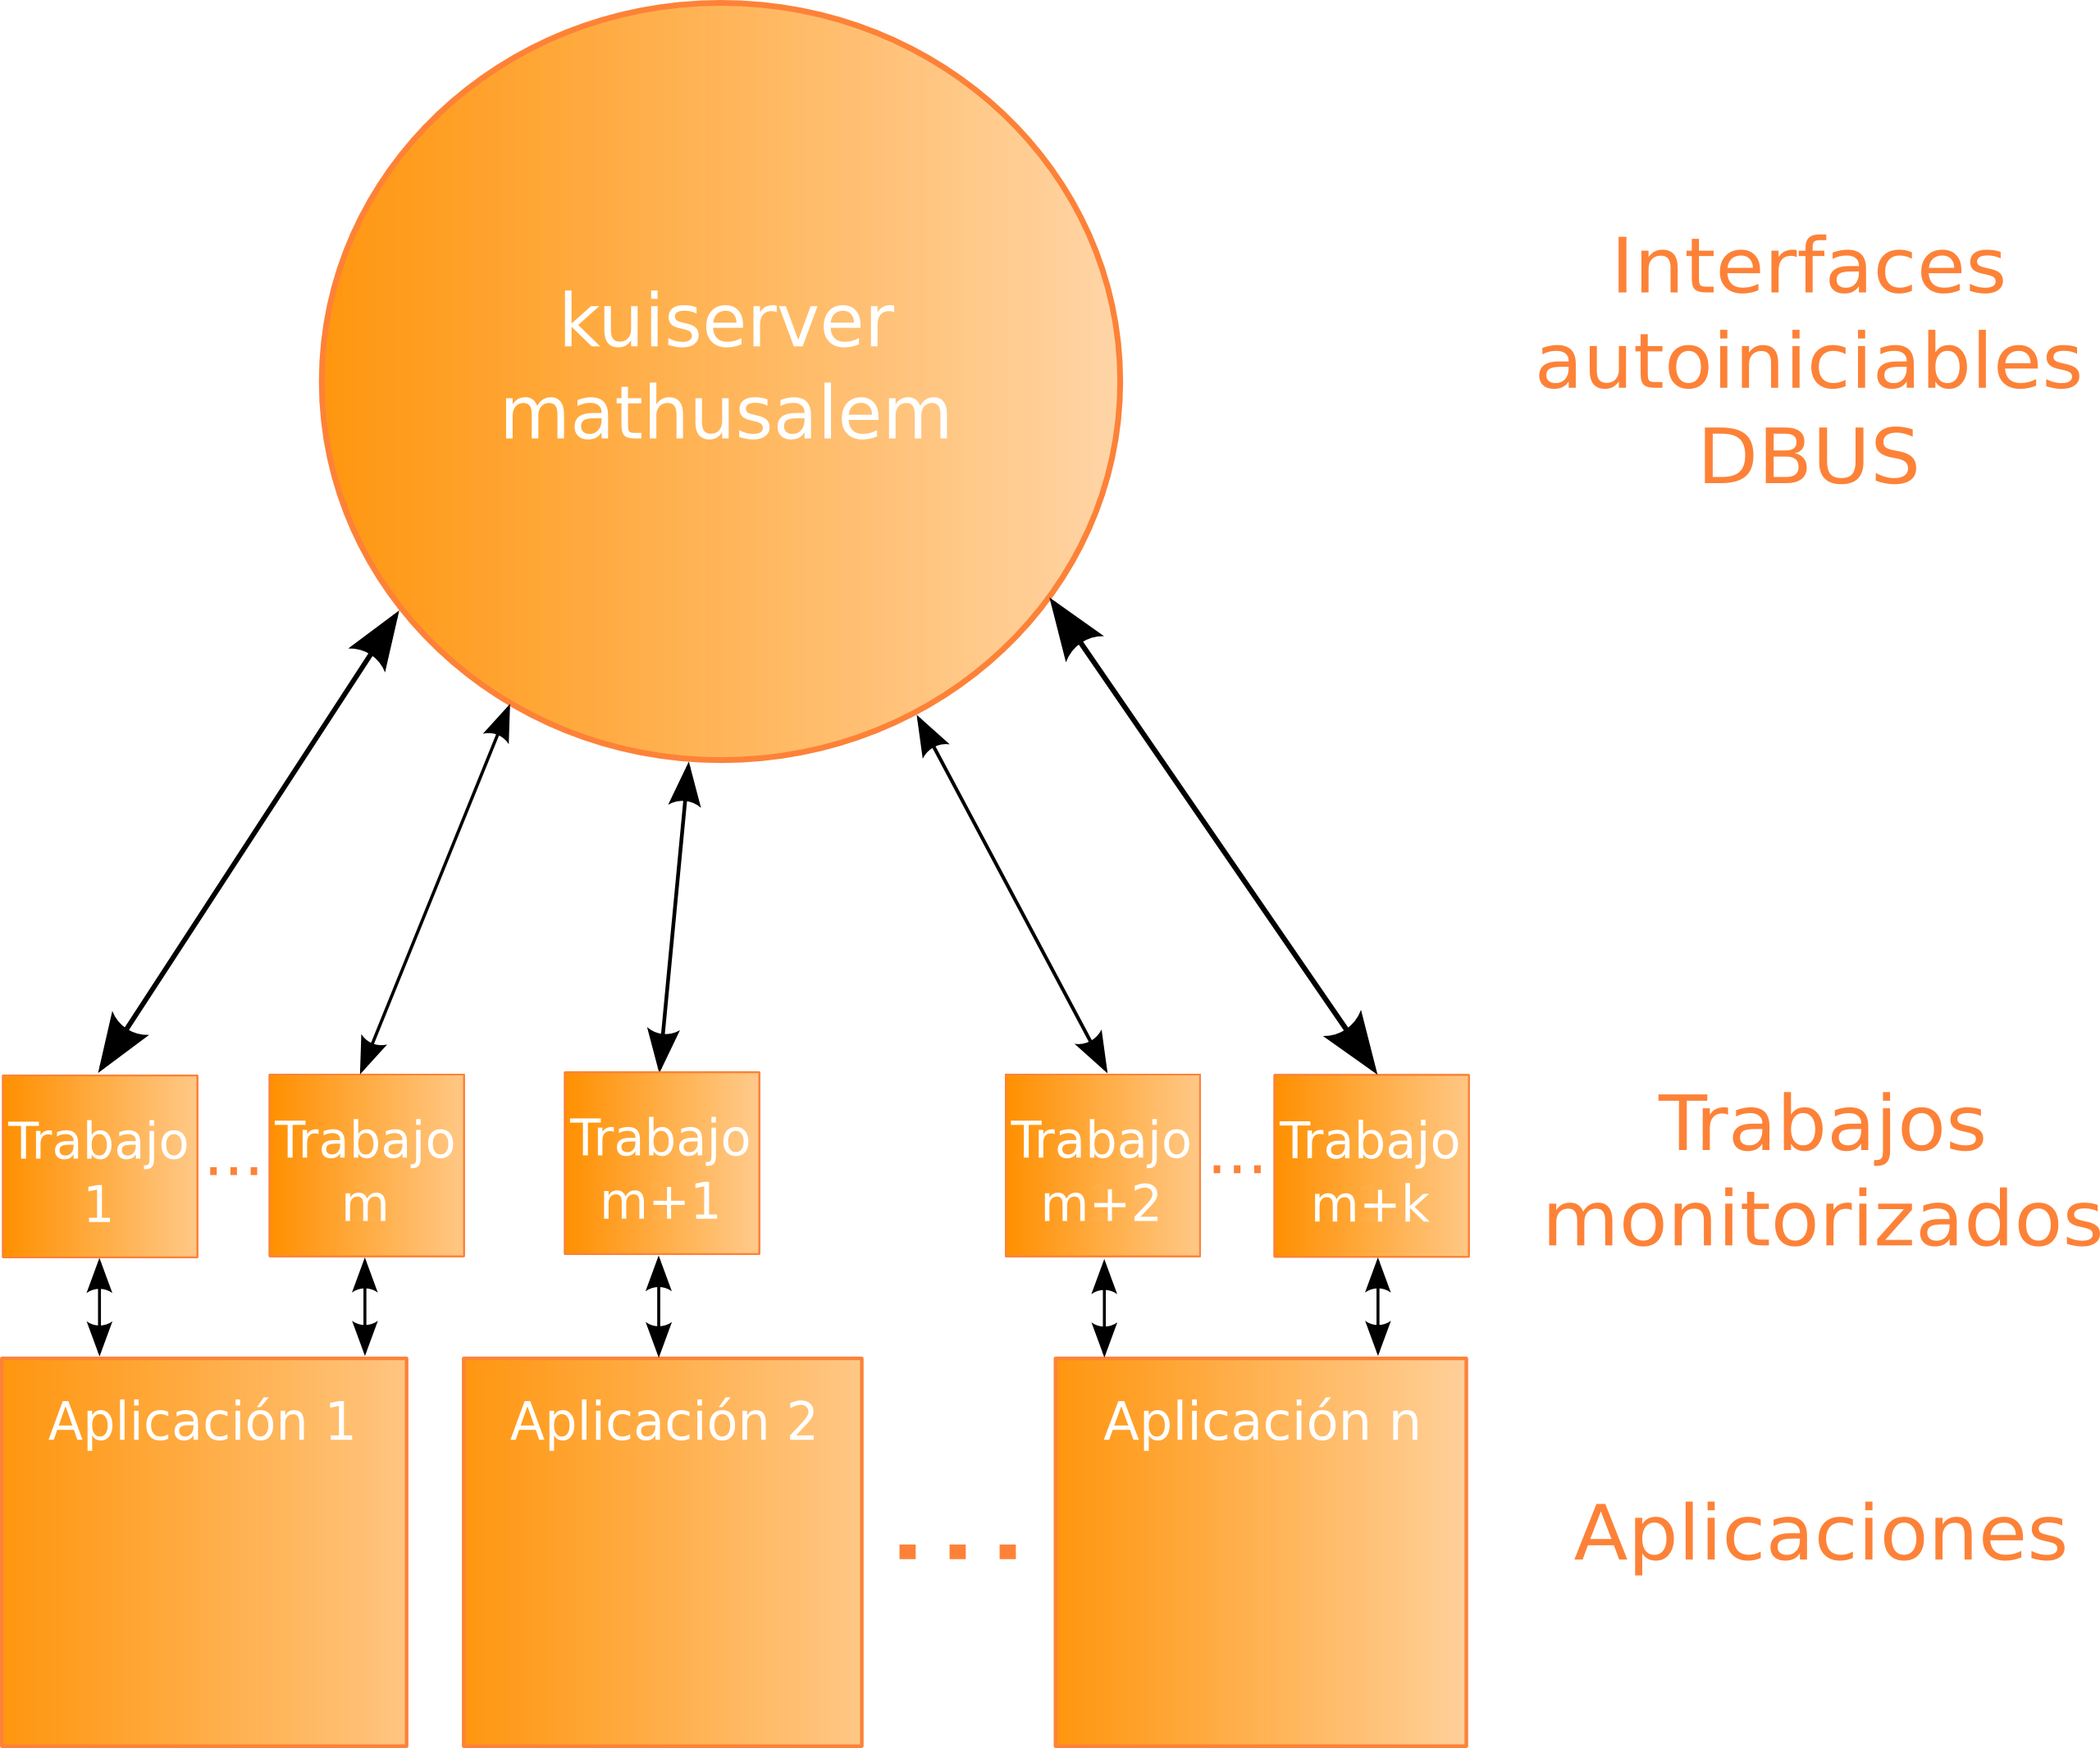
\includegraphics[width=9cm,height=7.5cm]{/home/geo/proyectos/charlas/kuiserver.png}
  \end{center}
\end{frame}

\begin{frame}
  \frametitle{KDE 3}
  \framesubtitle{kio\_uiserver}
  \begin{center}
    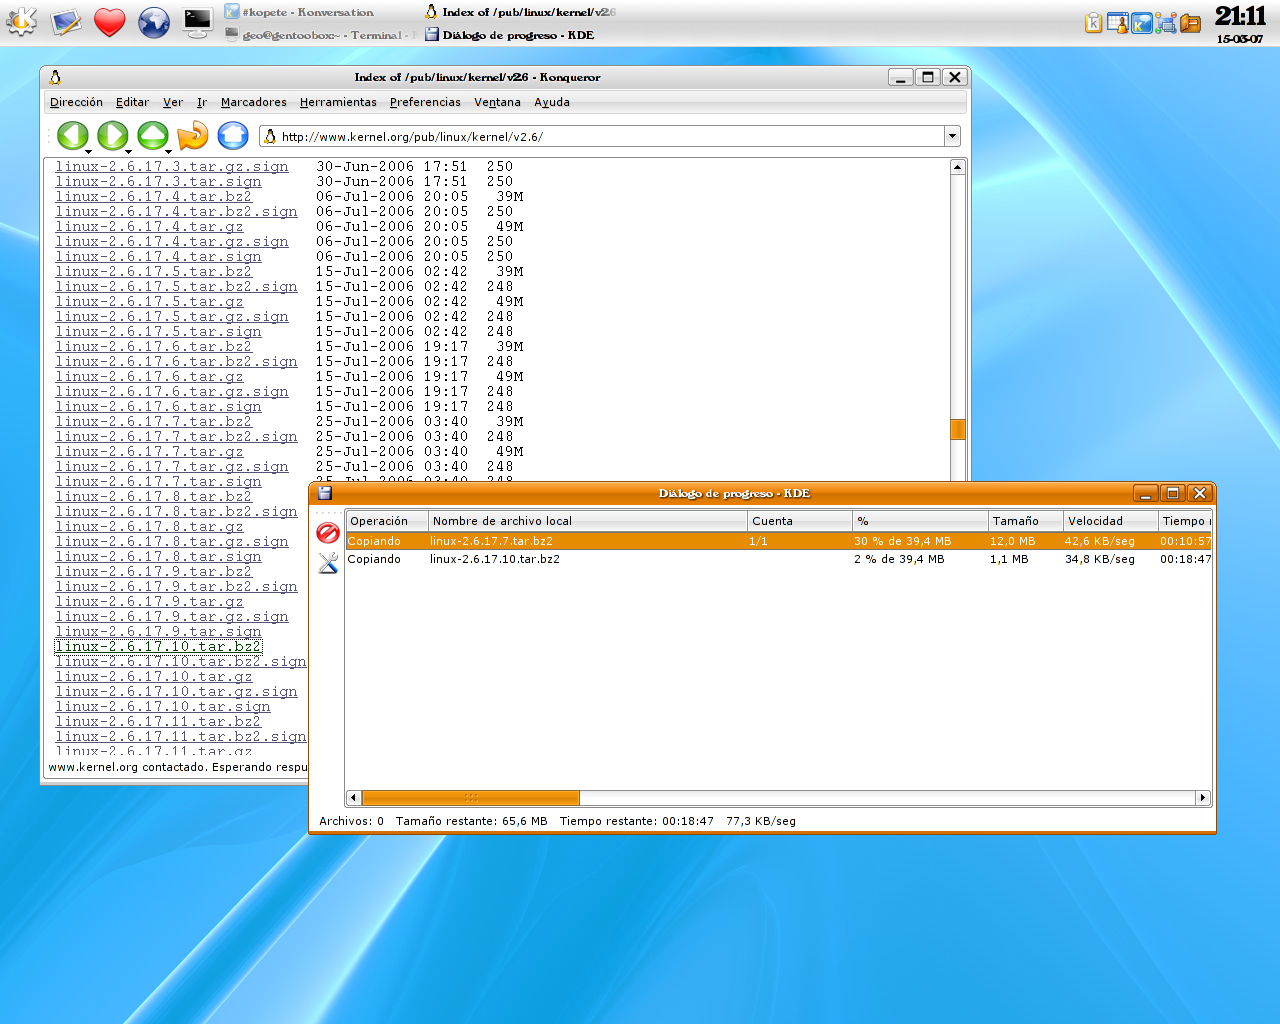
\includegraphics[width=10cm,height=7.5cm]{/home/geo/proyectos/charlas/kio_uiserver.png}
  \end{center}
\end{frame}

\begin{frame}
  \frametitle{KDE 3}
  \framesubtitle{kio}
  \begin{center}
    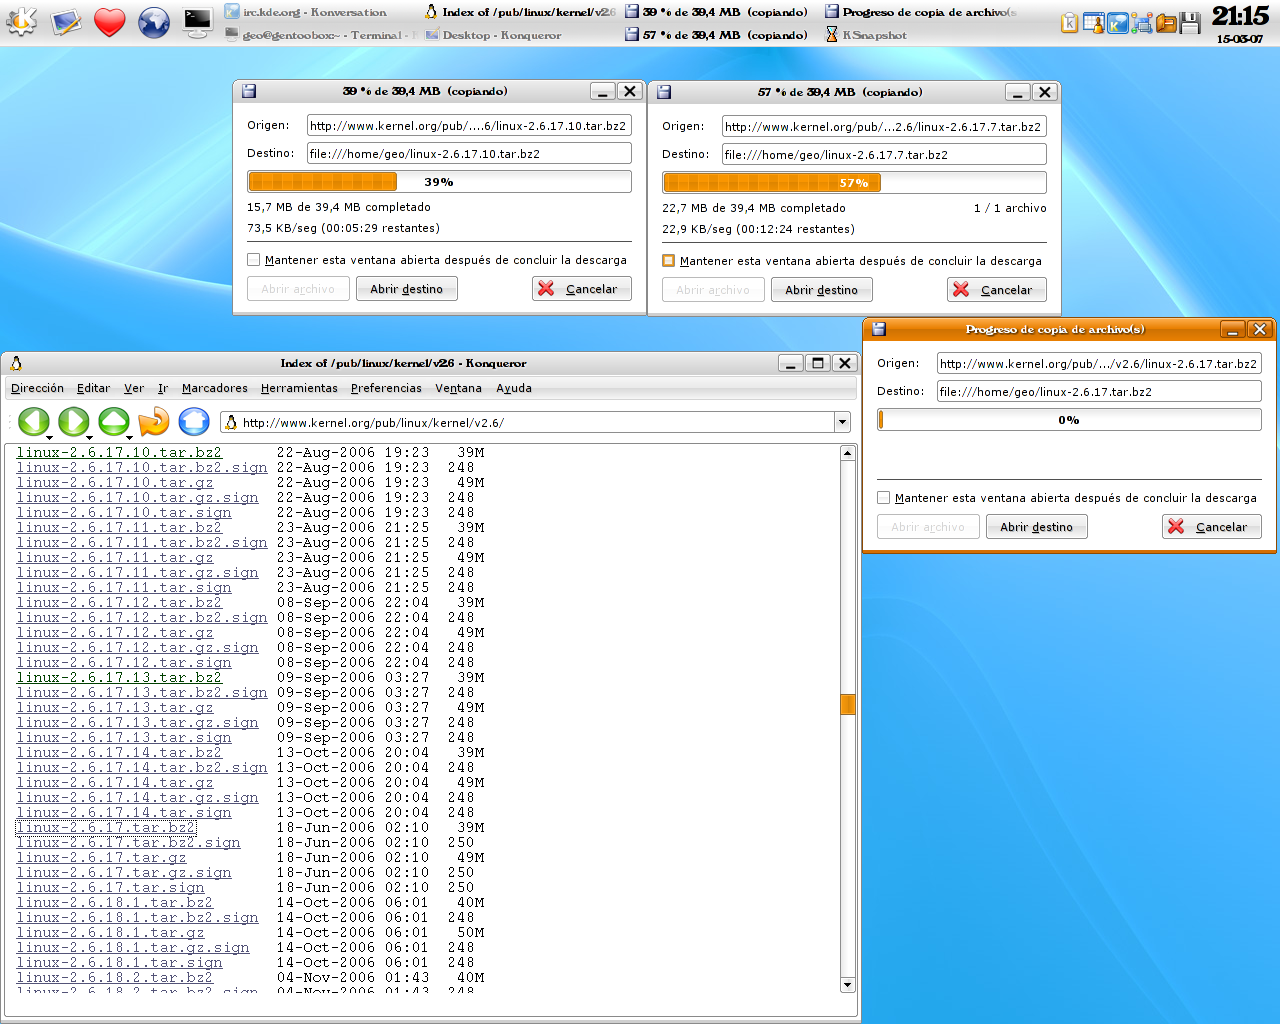
\includegraphics[width=10cm,height=7.5cm]{/home/geo/proyectos/charlas/kio_uiserver2.png}
  \end{center}
\end{frame}

\end{document}
